\documentclass[11  pt]{article}
\usepackage[lmargin=1in,rmargin=1.75in,bmargin=1in,tmargin=1in]{geometry}

% For hyperlinking everything
\usepackage{hyperref}
\hypersetup{
	colorlinks=true, %set true if you want colored links
	linktoc=all,     %set to all if you want both sections and subsections linked
	linkcolor=blue,  %choose some color if you want links to stand out
}


\usepackage[latin1]{inputenc}
\usepackage{amsmath}
\usepackage{mathrsfs}  
\usepackage{amsfonts}
\usepackage{amssymb}
\usepackage{graphicx}
\usepackage{subfig}
\usepackage{caption}
\usepackage{algorithm}
%\usepackage{algcompatible}
%\usepackage{algorithmicx}
\usepackage{algpseudocode}

\usepackage{titlesec}
\titleformat{\section}{\fontfamily{lmss}\fontsize{14}{15}\bfseries}{\thesection}{1em}{}
\titleformat{\subsection}{\fontfamily{lmss}\fontsize{12}{15}\bfseries}{\thesubsection}{1em}{}




\usepackage{amsthm}

\newtheoremstyle{noit}
{10pt}% <Space above>
{10pt}% <Space below>
{}% <Body font>
{}% <Indent amount>
{\bfseries}% <Theorem head font>
{.}% <Punctuation after theorem head>
{.5em}% <Space after theorem headi>
{}% <Theorem head spec (can be left empty, meaning `normal')>

\newtheoremstyle{example}
{10pt}% <Space above>
{10pt}% <Space below>
{}% <Body font>
{20pt}% <Indent amount>
{\bfseries}% <Theorem head font>
{.}% <Punctuation after theorem head>
{.5em}% <Space after theorem headi>
{}% <Theorem head spec (can be left empty, meaning `normal')>


\newtheoremstyle{indented}{20pt}{20pt}{\addtolength{\leftskip}{2.5em}}{}{\bfseries}{.}{.5em}{}


\newtheorem{theorem}{Theorem}
\numberwithin{theorem}{section}
\newtheorem{lemma}[theorem]{Lemma}
\newtheorem{corollary}[theorem]{Corollary}
\newtheorem{observation}{Observation}
%\numberwithin{observation}{section}
%\numberwithin{definition}{section}
\newtheorem{conjecture}{Conjecture}
\newtheorem{Qu}{Question}
\newcommand{\QU}{\begin{Qu}\normalfont}

\theoremstyle{noit}
\newtheorem{fact}{Fact}
\newtheorem{definition}{Definition}

\theoremstyle{indented}
\newtheorem{example}{Example}

\theoremstyle{indented}
\newtheorem{problem}{Problem}


%\newenvironment{proof}{\noindent{\bf Proof:} \hspace*{1em}}{
%    \hspace*{\fill} $\Box$ }
%\newenvironment{proof_of}[1]{\noindent {\bf Proof of #1:}
%    \hspace*{1em} }{\hspace*{\fill} $\Box$ }
%\newenvironment{proof_claim}{\begin{quotation} \noindent}{
%    \hspace*{\fill} $\diamond$ \end{quotation}}
\newcommand{\vs}[1]{\vspace{#1}}

\newcommand{\lecture}[2]{
 \noindent
\begin{center}
	\framebox{
		\vbox{
			\hbox to 5.78in { {\bf CSCE 411: Design and Analysis of Algorithms (Honors)} \hfill  }
			\vspace{2mm}
			\hbox to 5.78in { {\Large \hfill Lecture #1\hfill} }
			\vspace{2mm}
			\hbox to 5.78in { {\it Date: #2 \hfill Samson Zhou} }
		}
	}
\end{center}
\vspace*{4mm}
}

\newcommand{\week}[2]{
 \noindent
\begin{center}
	\framebox{
		\vbox{
			\hbox to 5.78in { {\bf CSCE 411: Design and Analysis of Algorithms (Honors)} \hfill  }
			\vspace{2mm}
			\hbox to 5.78in { {\Large \hfill Week #1\hfill} }
			\vspace{2mm}
			\hbox to 5.78in { {\it Date: #2 \hfill Nate Veldt, updated by Samson Zhou} }
		}
	}
\end{center}
\vspace*{4mm}
}

\newcommand{\sweek}[2]{
 \noindent
\begin{center}
	\framebox{
		\vbox{
			\hbox to 5.78in { {\bf CSCE 411: Design and Analysis of Algorithms (Honors)} \hfill  }
			\vspace{2mm}
			\hbox to 5.78in { {\Large \hfill Week #1\hfill} }
			\vspace{2mm}
			\hbox to 5.78in { {\it Date: #2 \hfill Samson Zhou} }
		}
	}
\end{center}
\vspace*{4mm}
}

\newcommand{\hw}[2]{
	\noindent
	\begin{center}
		\framebox{
			\vbox{
				\hbox to 5.78in { {\bf CSCE 411: Design and Analysis of Algorithms} \hfill  }
				\vspace{2mm}
				\hbox to 5.78in { {\Large \hfill Homework #1\hfill} }
				\vspace{2mm}
				\hbox to 5.78in { {\it Due date: #2 \hfil} }
			}
		}
	\end{center}
	\vspace*{4mm}
}



\newcommand{\under}[1]{\underline{\hspace{#1}}}
\setlength{\parindent}{0em}

%\usepackage[tagged]{accessibility}

% Graph terms
\newcommand{\vol}{\textbf{vol}}
\newcommand{\cut}{\textbf{cut}}


% Matrices
\newcommand{\mA}{\textbf{A}}
\newcommand{\mB}{\textbf{B}}

% vectors
\newcommand{\ve}{\textbf{e}}
\newcommand{\vx}{\textbf{x}}


% Other
\newcommand{\calN}{\mathcal{N}}

\usepackage{mathtools}
\DeclarePairedDelimiter\ceil{\lceil}{\rceil}
\DeclarePairedDelimiter\floor{\lfloor}{\rfloor}


\newcommand*{\aitem}{ \item[{
\includegraphics[width=0.8cm,height=0.5cm]{figures/A}} ]  }
\newcommand*{\bitem}{ \item[{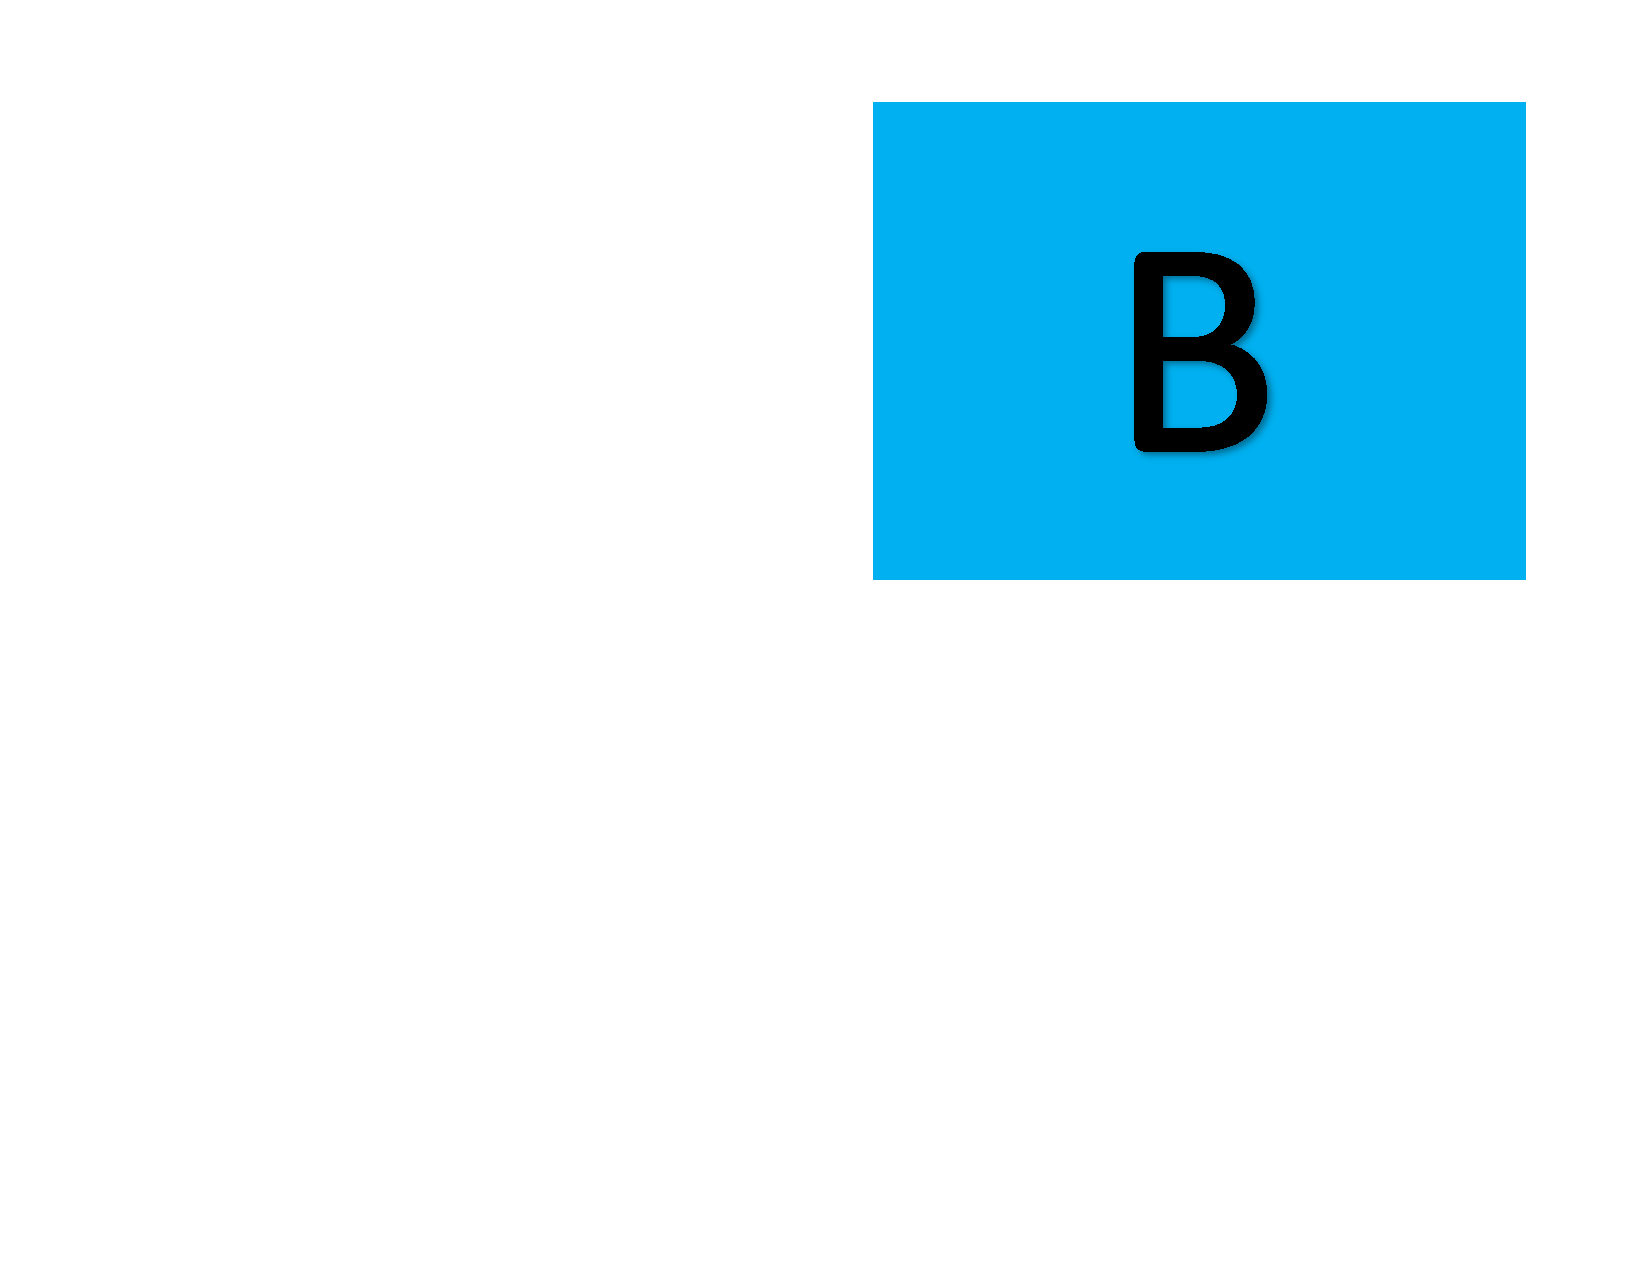
\includegraphics[width=0.8cm,height=0.5cm]{figures/B}} ]  }
\newcommand*{\citem}{ \item[{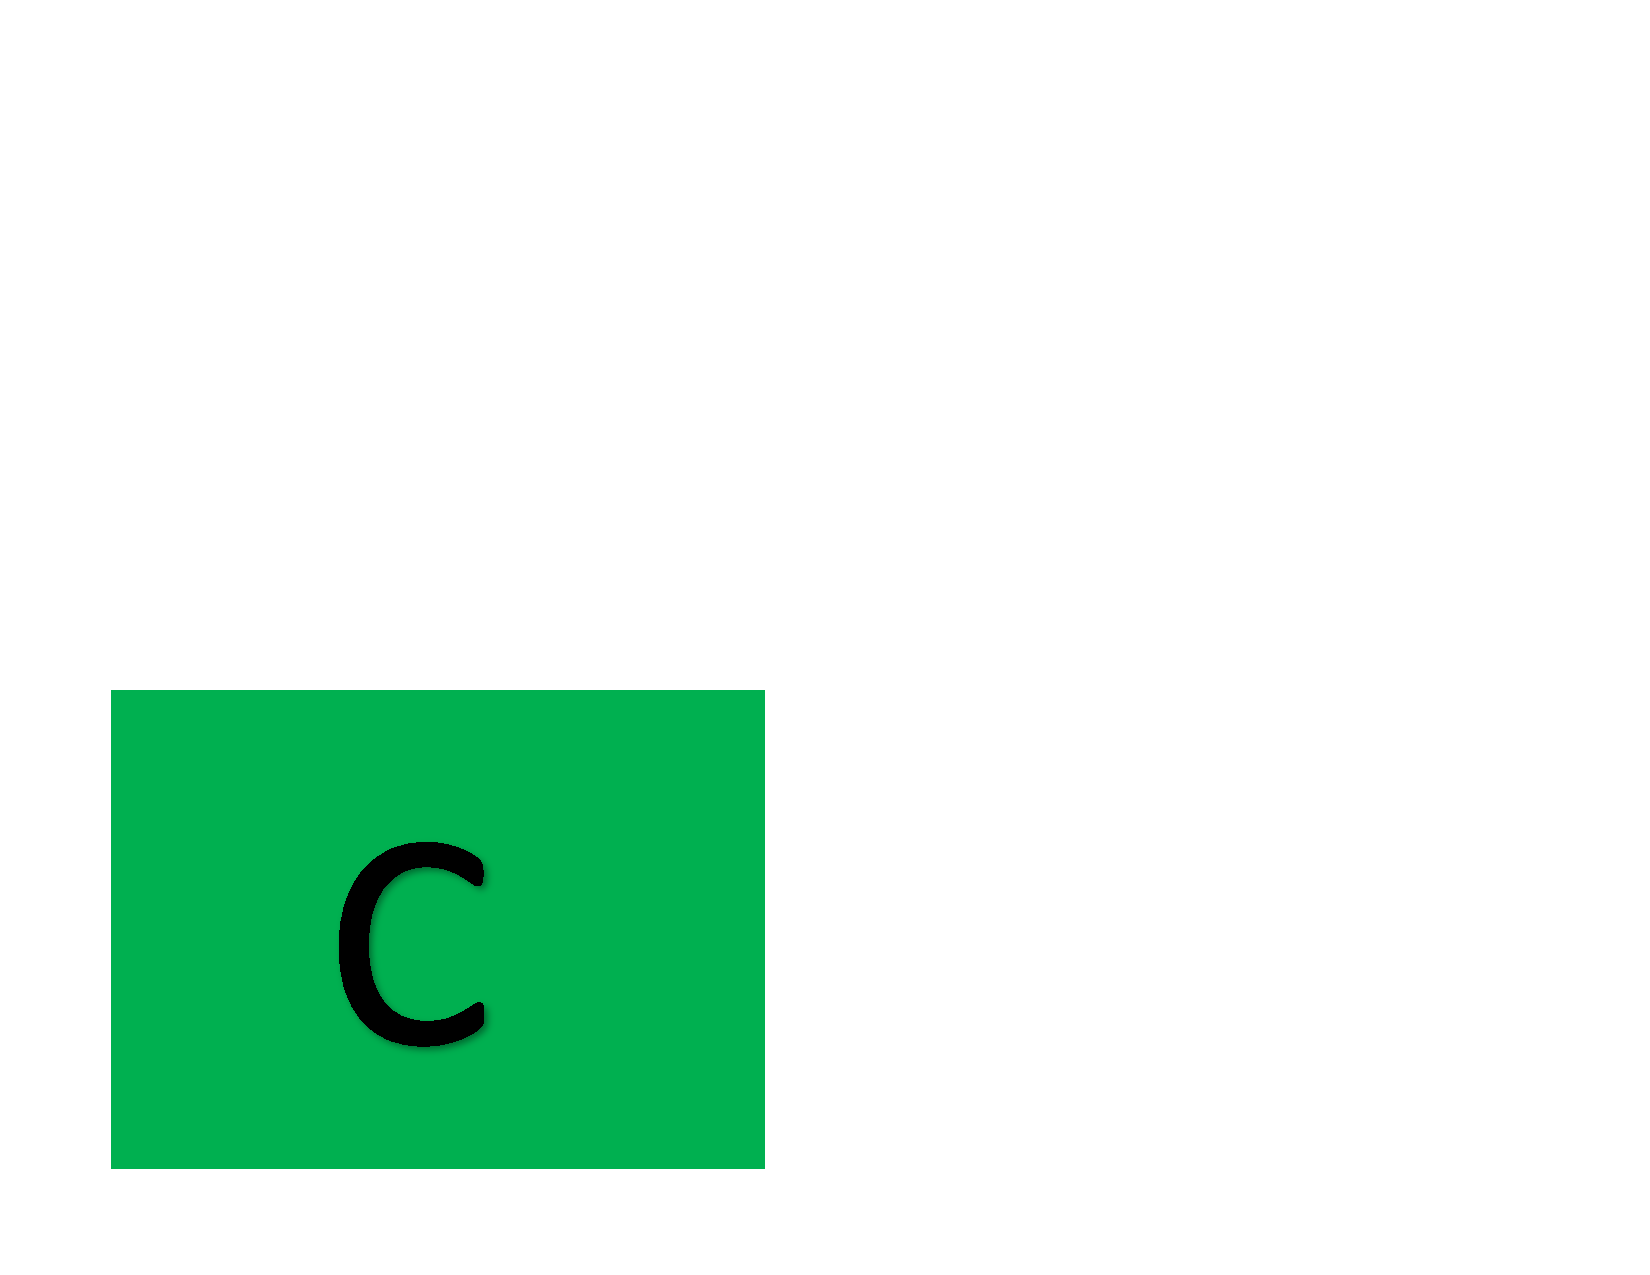
\includegraphics[width=0.8cm,height=0.5cm]{figures/C}} ]  }
\newcommand*{\ditem}{ \item[{
\includegraphics[width=0.8cm,height=0.5cm]{figures/D}} ]  }
\newcommand*{\eitem}{ \item[{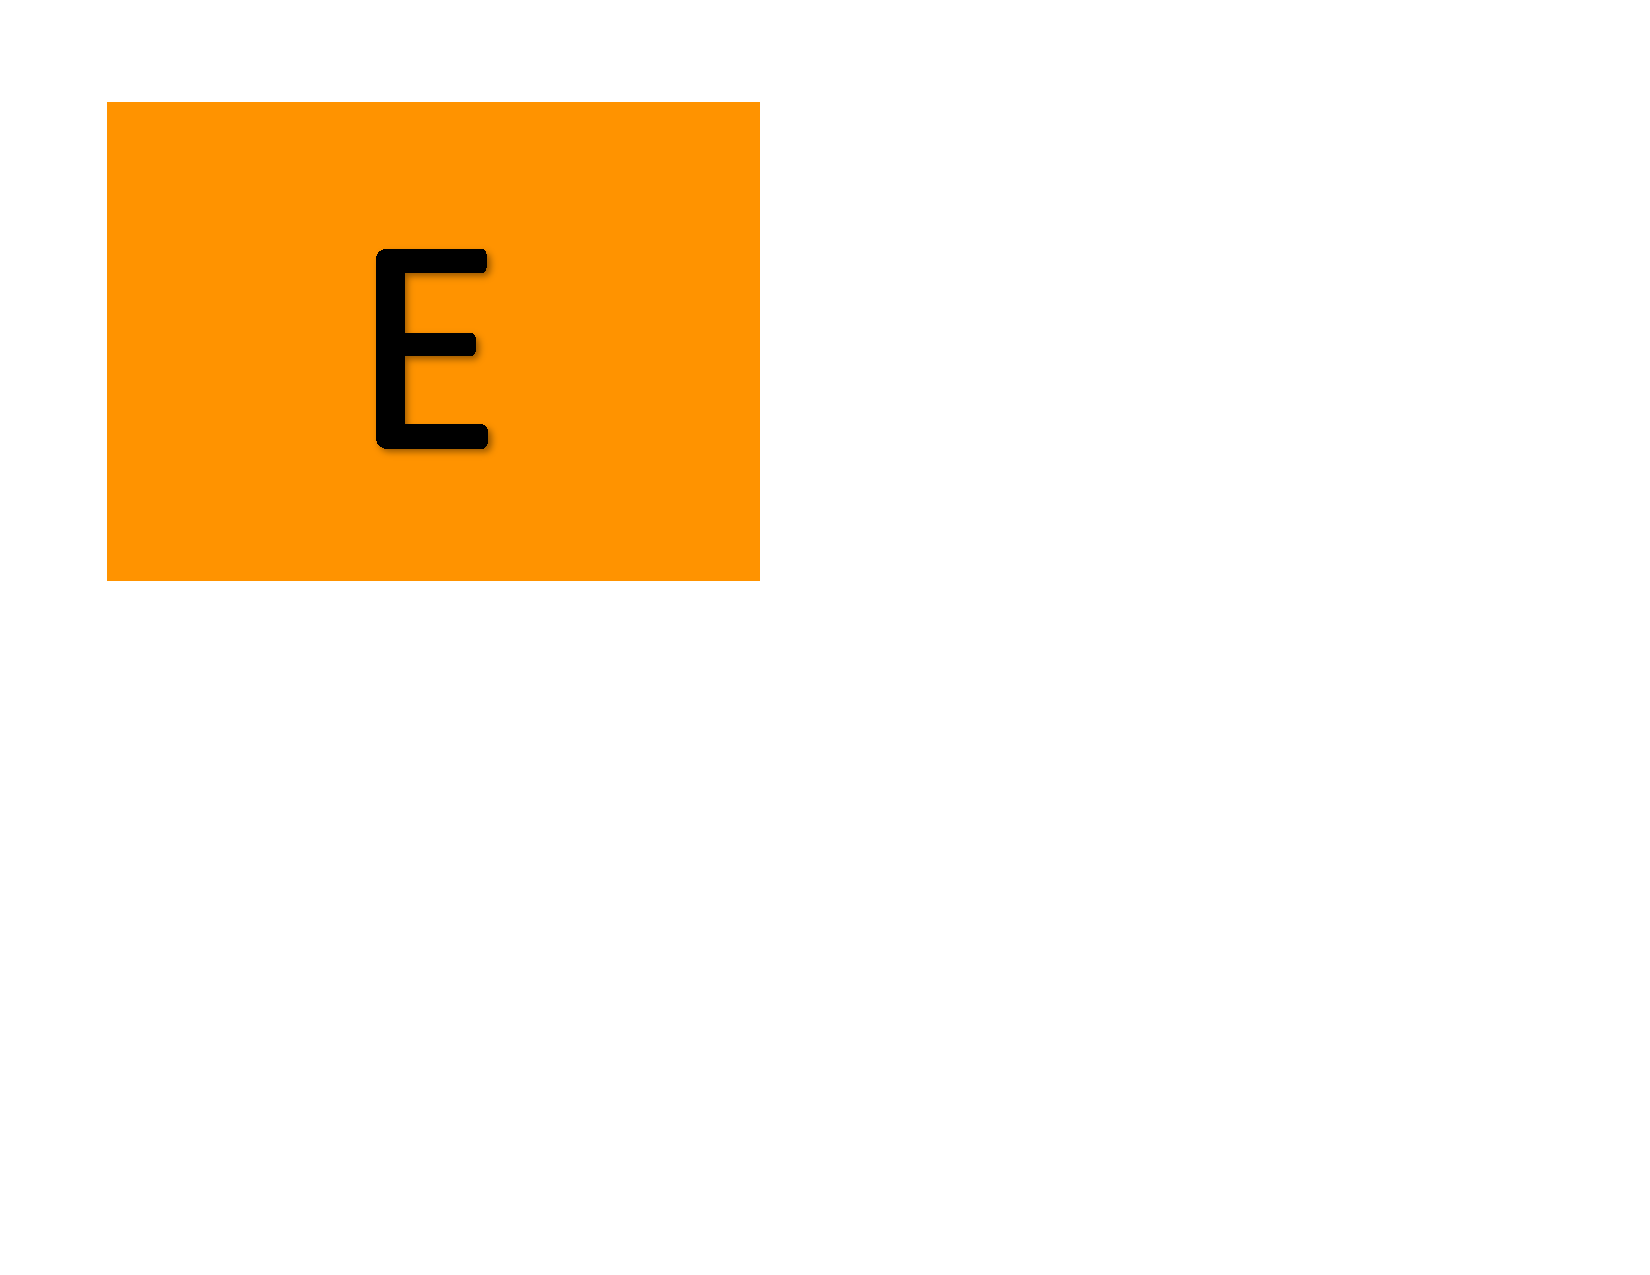
\includegraphics[width=0.8cm,height=0.5cm]{figures/E}} ]  }
\newcommand*{\fitem}{ \item[{
\includegraphics[width=0.8cm,height=0.5cm]{figures/F}} ]  }


\newcommand{\hide}[1]{\underline{\phantom{#1 #1}}}

\usepackage{setspace}

\onehalfspacing

\begin{document}
    \sweek{11: Input Representation and Undecidability}{November 5, 2026}
% Change the lecture label and date to match the course schedule.

\section{Prime Factorization and Primality Testing}
A positive integer $N\geq 2$ is \emph{prime} if its only positive divisors are \hide{$1$ and $N$.} An integer $N\geq 2$ that is not prime is called \emph{composite}.

\paragraph{Two different problems}
\begin{itemize}
    \item \textbf{Prime factorization:} Given $N\geq 2$, find the prime numbers whose product is $N$, including repeated factors.
    \vs{.5cm}
    \item \textbf{Primality testing:} Given $N\geq 2$, determine whether $N$ is prime.
\end{itemize}

\paragraph{Example}
What should each problem output on $N=91$? What about $N=97$?
\vs{2cm}
% 91 = 7*13, so primality testing answers NO.
% 97 is prime, so its factorization is just 97 and primality testing answers YES.

\begin{Qu}
    Which of the two problems is a decision problem as stated?
    \begin{itemize}
        \aitem Prime factorization
        \bitem Primality testing
        \citem Both
        \ditem Neither
    \end{itemize}
\end{Qu}
% Answer: (b). The factorization task asks for factors, not a YES/NO answer.

\vfill
\textbf{Observation.} A factorization can tell us whether a number is prime. A YES or NO answer about primality does not, by itself, supply the factors of a composite number.

\newpage
\subsection*{A simple algorithm}
We could test whether any integer between $2$ and $\lfloor\sqrt N\rfloor$ divides $N$.

\begin{algorithm}[h]
    \textsc{TrialDivision}($N$)
    \begin{algorithmic}
        \If{$N<2$}
            \State return NO
        \EndIf
        \State $d\gets 2$
        \While{$d^2\leq N$}
            \If{$d$ divides $N$}
                \State return NO
            \EndIf
            \State $d\gets d+1$
        \EndWhile
        \State return YES
    \end{algorithmic}
\end{algorithm}

\paragraph{Why is it correct?}
Suppose $N=ab$ with $a,b>1$. Why must at least one of $a$ and $b$ be at most $\sqrt N$?
\vs{1.5cm}
% If both were greater than sqrt(N), their product would be greater than N.

\begin{Qu}
    The algorithm tries at most $\sqrt N$ possible divisors. Does this show that primality testing has a polynomial-time algorithm?
    \begin{itemize}
        \aitem Yes, because $\sqrt N$ is bounded by a polynomial in $N$
        \bitem No, because the algorithm is incorrect
        \citem We must first determine the length of the input
    \end{itemize}
\end{Qu}
% Answer: (c). The algorithm is correct, but the relevant parameter is input length.

\vfill
\textbf{To be clear.} Starting at $1$ would not help: $1$ divides every integer. We are looking for a nontrivial divisor.

\newpage
\section{How Long Is the Input?}
The value of an integer and the length of its representation are different quantities. Let $N$ be the integer and $n$ the number of bits used to write it in binary, without leading zeros.

\paragraph{Warm-up}
Write $13$ in binary. How many bits did you use?
\vs{1cm}
% 13 = (1101)_2, which uses 4 bits.

An $n$-bit positive integer satisfies
\begin{equation*}
    2^{n-1}\leq N<2^n.
\end{equation*}
Therefore,
\begin{equation*}
    n=\hide{\lfloor\log_2 N\rfloor+1}.
\end{equation*}

\paragraph{Return to trial division}
On a prime input, the algorithm tests all candidates through $\lfloor\sqrt N\rfloor$. Express the number of candidates in terms of the input length $n$:
\begin{equation*}
    \sqrt N=\hide{\Theta(2^{n/2})}.
\end{equation*}
Is this polynomial or exponential in $n$?
\vs{1cm}
% Exponential. Even counting only the candidate tests already gives
% an exponential worst-case bound. Each divisibility test also has
% a bit-operation cost; elementary arithmetic takes polynomial time in n.

\paragraph{A numerical example}
For a prime with $100$ binary digits, the number of candidates is on the scale of $2^{50}$, which is about $10^{15}$. The input itself has only \hide{$100$ bits.}

\vfill
\textbf{Observation.} Polynomial time means polynomial in the \hide{length of the input}, not necessarily in the numerical value represented by the input.

\newpage
\subsection*{What if we change the representation?}
In unary, the integer $N$ is represented by $N$ copies of the symbol $1$.

\begin{Qu}
    If $N$ is given in unary, is trial division polynomial-time in the input length?
    \begin{itemize}
        \aitem Yes
        \bitem No
        \citem Only if $N$ is prime
    \end{itemize}
\end{Qu}
Explain why the answer differs from the binary case.
\vs{1cm}
% Answer: (a). The input length is now N. Reading the input and doing
% at most sqrt(N) divisions on O(log N)-bit values takes polynomial time in N.

\paragraph{Does a slow algorithm mean a hard problem?}
\begin{Qu}
    Does the running time of trial division prove that binary primality testing is not in $\mathrm{P}$?
    \begin{itemize}
        \aitem Yes
        \bitem No, because a different algorithm might be faster
    \end{itemize}
\end{Qu}
% Answer: (b).

\begin{theorem}[Agrawal--Kayal--Saxena]
    Primality testing is in \hide{$\mathrm{P}$.}
\end{theorem}
We will use this theorem without proving the algorithm. It concerns testing whether a number is prime; it does not itself give an algorithm for finding all prime factors.
% Reference: Agrawal, Kayal, Saxena, "PRIMES is in P", Annals of Mathematics
% 160 (2004), 781--793. https://annals.math.princeton.edu/2004/160-2/p12

\vfill
We have been asking whether a problem has an efficient algorithm. Next, we will ask a more basic question: does every decision problem have an algorithm at all?

\newpage
    \section{Decision problems and undecidability}
    A decision problem $Q$ is \emph{undecidable} if there cannot exist an algorithm that always halts and provides the correct YES or NO answer.

    \begin{Qu}
        Say that $Q$ is an NP-Complete problem. Which of the following statements is true?
        \begin{itemize}
            \aitem $Q$ is undecidable
            \bitem If $P \neq NP$, then $Q$ is undecidable, but we just do not know for sure yet
            \citem Neither of the above is true
        \end{itemize}
    \end{Qu}
    % Answer: (c). Enumerating all polynomial-length certificates gives
    % a decider, even if finding an accepting certificate takes a long time.


%\vfill
%Question: Are NP-hard problems the hardest problems that exist? Can anything be harder?
\newpage

\section{Halting and the Halting Problem}
Just as an integer can be represented by a string, the code of a program can also be represented by a string.

Let $P$ represent some notion of a computer program and $I$ represent some type of input that you give $P$. You can think of both as strings.\\

We say that $P$ \emph{halts} on $I$ if
\vs{2cm}
%\hide{running $P$ on input $I$ eventually terminates.} \\

\paragraph{Example}
Let $P = \textsc{OddHello}$ be represented by the following code snippet.
\begin{algorithm}[h]
    \textsc{OddHello}($I$)
    \begin{algorithmic}
        \If{the input is a string with an even number of letter characters (a-z)}
        \While{true}
        \State continue
        \EndWhile
        \Else
        \State return ``hello!''
        \EndIf
    \end{algorithmic}
\end{algorithm}
% iftheinputisastringwithanevennumberoflettercharactersazthenwhiletruedocontinueendwhileelseReturnHelloendif has 101 characters

\begin{Qu}
    Does $\langle P, I\rangle$ halt when $I$ = ``hello''?
    \begin{itemize}
        \aitem Yes
        \bitem Nope
        \citem It depends
        \ditem There is no way of knowing
    \end{itemize}
\end{Qu}
% Answer: (a).

\begin{Qu}
Does $\langle P, I\rangle$ halt when $I$ = ``hi''?
    \begin{itemize}
        \aitem Yes
        \bitem Nope
        \citem It depends
        \ditem There is no way of knowing
    \end{itemize}
\end{Qu}
% Answer: (b).

For the next question, suppose our fixed text representation of $P$ contains $101$ lowercase letters.
\begin{Qu}
    Does $\langle P, I\rangle$ halt when $I$ = $P$?
    \begin{itemize}
        \aitem Yes
        \bitem Nope
        \citem This question cannot have an answer
    \end{itemize}
\end{Qu}
% Answer: (a). A program description is a string and can be used as input.

\vspace{1cm}

\newpage

\textbf{Definition: The Halting Problem.} The \emph{halting problem} is a decision problem that takes in inputs of the form $\langle P, I \rangle$ and outputs
\begin{itemize}
    \item YES \\ \\%if P halts on I
    \item NO \\%if P does not halt on I
\end{itemize}

\emph{To be clear}
\begin{itemize}
    \item An instance of the halting problem is given by a \\ \\
    % program P and an input I.
    \item An algorithm $A$ solves the halting problem if
    % for every program-input pair (P,I), it halts and correctly answers
    % whether or not P halts on I.
\end{itemize}

\newpage

\begin{theorem} The Halting Problem is \hide{undecidable.}
\end{theorem}

\textit{Proof.} Suppose there is an algorithm $H$ that always halts and correctly solves the halting problem. Thus,
\begin{itemize}
    \item $H(M,I)$ returns YES if \hide{$M$ halts on $I$.}
    \item $H(M,I)$ returns NO if \hide{$M$ does not halt on $I$.}
\end{itemize}

We can represent the code of a program $M$ as a string $\langle M\rangle$. This string can also be used as the input to a program.

\paragraph{A new program}
Using $H$, construct the following program.
\begin{algorithm}[h]
    \textsc{Opposite}($z$)
    \begin{algorithmic}
        \If{$z$ is not a valid program description}
            \State return
        \EndIf
        \If{$H(z,z)$ returns YES}
            \While{true}
                \State continue
            \EndWhile
        \Else
            \State return
        \EndIf
    \end{algorithmic}
\end{algorithm}

\textbf{Observation.} Here $H(z,z)$ asks whether the program described by $z$ halts when its input is the string $z$.

\newpage
\subsection*{Running a program on its own description}
Let $b=\langle\textsc{Opposite}\rangle$ be the description of our new program. What happens when we run \textsc{Opposite}$(b)$?

\begin{itemize}
    \item Suppose $H(b,b)$ returns YES. What does $H$ predict, and what does \textsc{Opposite} actually do?
    \vs{2cm}
    % H predicts that Opposite(b) halts, but Opposite(b) loops forever.
    \item Suppose $H(b,b)$ returns NO. What does $H$ predict, and what does \textsc{Opposite} actually do?
    \vs{2cm}
    % H predicts that Opposite(b) does not halt, but Opposite(b) returns.
\end{itemize}

In either case, \hide{$H$ gives an incorrect answer.} Therefore, no such algorithm $H$ exists.

\paragraph{What if we impose a deadline?}
\begin{Qu}
    Given a program $M$, an input $I$, and a positive integer $T$, can an algorithm always decide whether $M$ halts on $I$ within $T$ steps?
    \begin{itemize}
        \aitem Yes
        \bitem No, because the halting problem is undecidable
        \citem Only if $M$ eventually halts on $I$
    \end{itemize}
\end{Qu}
% Answer: (a). Simulate M for T steps, stopping early if it halts.

\vfill
Next time, we will study how much memory a computation needs. Later, we will return to this deadline question and use it to prove a lower bound on running time.

\end{document}
